\chapter{The Taxation of Investment Income of Foreign Persons}

\intro{This chapter addresses the U.S. taxation of the investment income of foreign persons.  Foreign persons not engaged in a U.S. trade or business are taxed at a flat 30\% rate on U.S. source investment income such as interest, dividends, rents, and royalties, unless a treaty provision applies.  The 30\% tax is collected by the U.S. person who pays the income to the foreign investor.  This chapter also discusses the source of income rules for non-investment income.  The source of income rules are also important for U.S. persons who earn foreign income as the rules determine tthe U.S. person's foreign tax credit limitation.  Finally, the U.S. withholding rules are briefly mentioned, and the applicable treaty provisions are also discussed.}
    
Foreign persons---both individuals and corporations---not engaged in a U.S. trade or business are taxed on U.S. source income that is fixed, determinable, annual or periodical (``FDAP'') at a flat, 30\% rate. \S\S 871(a)(1) (individuals) and 881(a)(1) (corporations).  \margit{Foreign persons are taxed on U.S. source FDAP at a flat 30\% rate.}FDAP includes most categories of periodic investment income, such as interest, dividends, rents, and royalties, as well as once-in-a-lifetime income, such as lottery winnings.  Importantly, most U.S. source interest, such as interest on bank deposits and ``portfolio interest,'' is exempt from U.S. tax.  In addition, most capital gains arising from the sale of U.S. assets by foreigners, except for gains from U.S. real estate, are not FDAP and are therefore exempt from U.S. tax.  The tax on FDAP income is collected by the last U.S. payor withholding the statutory percentage (generally 30\%) from the income.  \S\S 1441(a), 1442(a)(1).  Treaties significantly reduce or eliminate source basis taxation on FDAP income.  For example, in almost all U.S. treaties, the source country tax on interest and royalties is reduced to 0\%, and the tax on dividends is reduced to a maximum of 15\%. 

The statutory regime requires the following analysis to determine the substantive tax liability of a foreign person not engaged in a U.S. trade or business:  First, the character of the income must be determined, \emph{e.g.}, dividend, interest, or royalty.  This is done under U.S. tax principles.  (Note the income may have a different character under U.S. law than under the law of the residence country.)  \margit{Tax algorithm: character, source, taxation under the Code, and application of a treaty.} Next, the income's source must be determined.  The source rules---found in sections 861, 862, 863, and 865---assign a source, U.S. or foreign, to most common categories of income, gains, deductions, and losses for both U.S. and foreign persons.  If the income is U.S. source FDAP, the income will be subject to a flat 30\% tax unless the income is exempt, for example, because it qualifies as portfolio interest under \S 871(h).  If the income is not exempt, withholding at 30\% will generally be required by the U.S. payor, unless a treaty reduces or eliminates U.S. tax. 

The source of income rules are the bedrock of the U.S. international tax regime.  For foreign persons, the U.S. generally limits its tax jurisdiction to items that are U.S. source, both for investment and for business income.  With respect to U.S. persons, the source rules primarily apply in determining a taxpayer's foreign tax credit limitation. \emph{See} \S\S 901 and 904.  U.S. persons are taxed on their worldwide income.  If a foreign jurisdiction also taxes a U.S. person's income, the taxpayer may elect to credit foreign taxes paid against his U.S. tax liability, subject to certain limitations.  Under \S 904, the amount of foreign taxes that can be credited against a taxpayer's federal (pre-credit) income tax liability is limited to the ratio of foreign source taxable income to worldwide taxable income times the U.S. tax liability (before any credits):  

\begin{center}
\begin{framed}
\begin{equation*}
\text{\emph{FTC  Limit}} = \frac{\text{Foreign Source Taxable Income}}{\text{Worldwide Taxable Income}} * \text{U.S. Tax (Pre-Credit)}
\end{equation*}
\end{framed}
\end{center}

Thus, the greater the proportion of foreign source income, the greater the foreign tax credit limit.  Treaties may modify the domestic foreign tax credit rules by providing treaty-specific source rules that modify the source rules under the IRC.

The materials that follow in this chapter explore the statutory source rules and FDAP regime.  Because, however, the source of income rules also arise in the context of the foreign tax credit of U.S. persons and the taxation of U.S. business income of foreign persons, some materials refer to those provisions.  

\section{Interest and Dividends}
\crt{861(a)(1), (2); 862(a)(1); 871(a), (h), (i), and (k); 881(a)(1) and (c); 1441(a); and 1442(a)}{1.861-2(a)(2), (7); 1.861-3(a)(6); 1.863-7; 1.871-7(b)(2); 1.871-14(g); 1.894-1(c); 1.1441-1(a) and (b); and 1.441-2(b)(2)(i)}{Articles 10 and 11}

% \addcontentsline{toc}{section}{\protect\numberline{}Interest} 
%\begin{center}
%\textbf{Interest}
	\subsection{Interest}
%\end{center}

Interest paid by a U.S. person is generally U.S. source FDAP.  \S 861(a)(1).  Thus, interest paid by U.S. individuals, U.S. corporations, and federal, state, and local governments is generally \margit{Interest paid by U.S. persons is generally U.S. source.}U.S. source.\footnote{Prior to 2010, if 80\% or more of the gross income of a resident alien or U.S. corporation was \emph{active foreign business income}, the interest paid was foreign source.  Former \S861(a)(1)(A). This rule, known as the 80/20 company rule, was repealed in 2010 in P.L. 111-226 (Education Jobs and Medicaid Assistance Act).  Certain existing 80/20 companies were grandfathered under section 871(l), and the active foreign business percentage of any interest paid by such companies is exempt under section 871(i)(2)(B)(ii). }    

%This rule,, perhaps reflects the notion that interest is paid from income generated by a person's assets, and if a very significant portion of a person's income is foreign source because his assets are employed abroad, any interest paid should also be foreign source.  If the interest is received by a related person (10\% or more ownership), only a percentage of the interest paid will be foreign source.  This percentage is equal to the ratio of foreign source income to total gross income over the 3-year testing period.  \S\S 871(i)(2)(D); 881(d).    In the President's Fiscal Year 2010 Budget Proposal, the 80/20 company rule was proposed to be repealed.  

Interest paid by a foreign branch of a U.S. commercial bank or savings and loan institution is foreign source. \S861(a)(1)(A)(i) and (ii).  Since commercial banks generally conduct business through branches, in the absence of this rule, interest paid on deposits would otherwise be U.S. source FDAP potentially subject to U.S. tax.  U.S. banks operating abroad would therefore be at a competitive disadvantage vis-a-vis local branches of foreign banks.  

Interest paid by a U.S. branch of a foreign corporation is U.S. source.  \S884(f)(1).  In addition, interest paid by a foreign partnership that is engaged in a U.S. trade or business (but predominantly engaged in the active conduct of a trade or business outside of the United States) is U.S. source to the extent that the interest is allocable to income that is treated as effectively connected with the U.S. trade or business.  \S861(a)(1)(B).

Even if interest is U.S. source, very little U.S. source interest paid to foreign persons is subject to U.S. tax under section 871 (or 881) because of the exemptions for portfolio interest and bank deposit interest.  \S\S 871(h) and (i)(2); 881(c) and (d).  \margit{U.S. source portfolio interest and bank deposit interest is exempt from tax.}Portfolio interest covers virtually any interest on registered debt except interest on bank deposits and interest received by a shareholder (or partner) owning 10\% or more of the payor corporation (or partnership).  Bearer (unregistered) debt issued prior to March 19, 2012, can also qualify for the portfolio interest exemption, provided that it was issued abroad to foreign persons.  \S871(h)(1)(2)(A). In addition, certain categories of contingent interest, such as interest tied to an obligor's cash flow, sales, or income, do not qualify as portfolio interest. \S871(h)(4).  

Because interest is deductible by the debtor and not taxable in the hands of foreign creditors, the portfolio interest exemption permits returns on U.S. business income paid out as interest to escape U.S. tax.  This rule may encourage U.S. businesses funded by foreign capital to be more highly leveraged than they would be otherwise.  Although such interest would not qualify as portfolio interest (if it's paid to a 10\%-or-great shareholder), under almost all U.S. treaties, interest is not subject to source basis taxation regardless of the ownership percentage of the recipient.  To protect the U.S. tax base from excessive debt held by foreign creditors, Congress enacted section 163(j), which restricts the deduction of interest paid by highly leveraged U.S. entities to certain foreign persons (and other tax-exempt entities).  Section 163(j) is discussed below in Chapter 6.3.

Under Article 11, interest generally cannot be taxed by the source country.  \margit{Treaties generally eliminate source basis taxation of interest.}Thus, the 10\% shareholder limitation of the portfolio interest rules is eliminated under the Treaty. Contingent interest can be taxed by the source country but only at a maximum rate of 15\%.  \emph{See} Article 11(5). 
 
The portfolio interest rules were originally enacted in 1984.  One issue that subsequently arose in conjunction with the growth of hedge funds and the expansion of their investing activities was whether in the case of debt held by a partnership, the 10\% shareholder rule would apply at the partner or partnership level.  In 2007, the Treasury issued final regulations that apply the 10\% shareholder test at the partner level rather than partnership level.  Reg.\@ \S 1.871-14(g)(3).  For example, if a partnership has 20 equal unrelated partners and the partnership owns 100\% of the U.S. payor corporation, all of the interest will be portfolio interest because no partner will own indirectly more than 10\% of the payor corporation.  The rationale for this treatment is that since the foreign partner is the beneficial owner of the interest, the portfolio interest rule should be tested at the partner level.   


%The preamble to the proposed regulations excerpted below describes the rationale for adopting this approach.      
%  \addcontentsline{toc}{section}{\protect\numberline{}Excerpt from the Proposed Portfolio Interest Regulations} 
%\begin{select}
%\revrul{Excerpt from the Preamble to the Proposed Portfolio Interest Regulations (Prop. Reg.\@ \S 1.871-14(g))}{June 13, 2006 (issued in final in T.D. 9323 (4/12/07)}
%\begin{center} \textbf{2. Person Who ``Receives" Interest for Purposes of the 10-percent Shareholder Test}
%\end{center}
%Section 871(h)(3) generally provides that interest received by a 10-percent shareholder is not considered portfolio interest exempt from taxation. When a partnership with foreign partners holds a debt instrument, the issue arises as to whether the withholding agent should apply the 10-percent shareholder test at the partner level (because such partner is the beneficial owner of the interest within the meaning of \S1.1441-1(c)(6)), at the partnership level (because the partnership holds the debt instrument), or at both levels. \ldots

%After considering the alternatives, the IRS and the Treasury Department conclude that the 10-percent shareholder test should apply at the foreign partner level to the nonresident alien individual or foreign corporation that is the beneficial owner of the income. Accordingly, the proposed regulations provide that when interest is paid to a partnership, the persons who receive the interest for purposes of applying the 10-percent shareholder test are the nonresident alien individual partners and the foreign corporations that are partners in the partnership. The 10-percent shareholder test is then applied by determining each such person's ownership interest in the obligor. No inference is intended as to whether other limitations set forth in the definition of portfolio interest should be considered at the partner level, partnership level, or at both levels (section 881(c)(3)(A)).

%The approach taken in the proposed regulation is supported by the statute and legislative history which convey Congress' desire to facilitate the efficient and effective flow of foreign capital to U.S. borrowers while distinguishing true portfolio investors in the obligor from foreign persons making direct (ten percent) equity investments in U.S. operations. \ldots With regard to the statute, it is clear from subchapter K, section 871, and section 881 that, in the absence of the portfolio interest exception, the tax on interest paid to a partnership is substantively imposed on the nonresident alien individual or foreign corporation that is a partner in the partnership. That is, the beneficial owner with respect to interest paid to a partnership is the foreign partner (other than a partner that is itself a passthrough entity) and not the partnership. Based upon this fact, the IRS and the Treasury Department believe that applying the 10-percent shareholder test in section 871(h)(3) at the partner level is consistent with the statutory framework of sections 871(h)(1) and 881(c)(1) which provide that portfolio interest ``received by a nonresident individual'' or ``received by a foreign corporation,'' respectively, from sources within the U.S. is exempt from taxation under sections 871(a) and 881(a).

%Further, notwithstanding the general regime for imposing tax under sections 871 and 881, the IRS and the Treasury Department do not believe that in enacting the 10-percent shareholder test, Congress intended for the test to be applied at the partnership level. Such an interpretation would condition a foreign beneficial owner's entitlement to the portfolio interest exception on the ownership in the obligor held by either a person that is not a taxpayer (the partnership) or a person who is wholly unrelated to the beneficial owner (another partner in the partnership). The practical effect of this interpretation would be to characterize interest payments made to a partnership as being received by a 10-percent shareholder in many cases where there is no apparent abuse, thereby disallowing a tax benefit to foreign persons, and impairing the free-flow of foreign capital to U.S. business, solely because a foreign person acted indirectly rather than directly with its U.S. borrower. For example, if 100 unrelated nonresident alien individuals and foreign corporations invest in a partnership that holds 10 percent of a domestic corporation, and such domestic corporation pays U.S. source interest to the partnership, each of the foreign partners in the partnership would be denied the benefit of the portfolio interest exception if the 10-percent shareholder test is applied at the partnership level. The same result occurs if unrelated U.S. persons that are partners in the partnership hold, in combination with the partnership, 10-percent of the domestic corporate obligor. The IRS and the Treasury Department believe that such a result is inapposite to the statutory framework and underlying purpose of the statute, especially considering that section 871(h) invokes the attribution rules of section 318 for the purpose of policing the 10-percent shareholder prohibition, and generally liberalizes the application of such rules to reach more subtle ownership arrangements.

%\ldots
%\end{select}
 
 
% \addcontentsline{toc}{section}{\protect\numberline{}Dividends} 
%\begin{center}
%\textbf{Dividends}
	\subsection{Dividends}
%\end{center}

Dividends paid by U.S. corporations are U.S. source FDAP.  \S 861(a)(2)(A).  \margit{Dividends from U.S. corporations and some foreign corporations are U.S. source.} Dividends paid by a \emph{foreign} corporation can also be U.S. source.  In particular, if 25\% or more of a foreign corporation's gross income over the three years preceding the year in which the dividend is paid is effectively connected income under section 864, a dividend from the corporation will be U.S. source in the same proportion as the effectively connected income.  \S 861(a)(2)(B).   

The goal of this provision was to equalize the aggregate tax paid on U.S. business profits whether the business was operated directly through a U.S. branch or indirectly through a U.S. subsidiary.  Congress revised the taxation of U.S. branches of foreign corporations in 1986 with the enactment of the branch profits tax (\emph{see} \S884), but did not repeal the secondary level withholding tax of section 861(a)(2)(B).  Since the enactment of the branch profits tax, U.S. business income earned by a branch is taxed when earned at graduated rates and again at a flat 30\% when the business profits are deemed distributed.  Thus, U.S. business income is taxed twice whether earned by a branch or U.S. subsidiary.  Dividends paid by a foreign corporation subject to the branch profits tax, however, are not taxed again as FDAP.  \S884(e)(3)(A). The branch profits tax is discussed below in Chapter 4.3. 

Foreign countries did not take kindly to the United States attempting to tax dividends paid by their corporations to their residents, and if a country had a tax treaty with the United States, the treaty invariably exempted such dividends from U.S. tax.  Furthermore, given the administrative difficulties in collecting U.S. tax on dividends paid by foreign corporations, it is probably not too much of a stretch to assume that this tax raised very little revenue.  Consequently, Congress eliminated in 2004 the 30\% FDAP tax on such dividends but left intact the dividend sourcing rule. \S\S 871(i)(2)(D); 881(d).\footnote{Prior to 2011, certain dividends paid by a 80/20 company, although U.S. source, were exempt from U.S. tax under section 871.  Former \S\S 871(i)(2)(B); 881(d).  In P.L. 111-226 (Education Jobs and Medicaid Assistance Act), the 80/20 rules were repealed, but certain existing 80/20 corporations are grandfathered.  The active foreign business percentage of any dividend paid by these corporations are exempt from tax. \emph{See} \S\S871(i)(2)(B)(i) and (l).} 

Under the Treaty, source basis taxation of dividends is generally not entirely eliminated.  \margit{Treaties reduce the 30\% rate to 15\%, 5\%, and sometimes 0\%.}Under Article 10(2), dividends are taxed at 15\% unless the beneficial owner owns directly or indirectly at least 10\% of the voting power of the corporation paying the dividend, in which case the rate drops to 5\%.  Notably, Article 10(3) provides for a 0\% rate on dividends received by either: (1) a company owning 80\% or more of the dividend paying corporation for the 12-month period ending on the dividend declaration date; or (2) a pension plan.  

A corporation is eligible for treaty benefits only if it is a \emph{resident} under Article 4 and a \emph{qualified person} under Article 23 (Limitations on Benefits).  The Limitation on Benefits article is discussed in more detail below at Chapter 6.2.  A company can satisfy the qualified person requirements in various ways.  A company can be a qualified person if its shares are traded on an exchange of one of the treaty signatories (publicly traded test).  A corporation can be a qualified person if other qualified persons own 50\% or more of the vote and value of the corporation and less than 50\% of the company's gross income is payable as a deduction to non-treaty residents (ownership-base erosion test).  A corporation can also be a qualified person if 95\% or more of its vote and value is owned by 7 or fewer persons who are residents of the EC, EEA, Canada, or Mexico (derivative benefits test).  Finally, a corporation not satisfying any of the above tests can obtain treaty benefits with respect to income or gain arising in the other contracting state if the corporation is engaged in the active conduct of a trade or business in the other state (active business test).  

To prevent companies from inappropriately restructuring their operations to become eligible for the 0\% inter-company dividend rate, the Treaty imposes additional restrictions beyond those of Article 23.  In particular, if the company receiving the dividend is a qualified resident under only the \emph{active trade or business} or \emph{ownership-base erosion} test, the dividend recipient must have acquired the 80\%-or-more ownership interest before October 1, 1998.  This was the first U.S. tax treaty to provide for a zero rate of tax on inter-company dividends; subsequent treaties generally provide for a zero rate in similar circumstances.  A few other treaties had previously provided for a zero rate on dividends, but only for dividends paid to pension plans.   

%\addcontentsline{toc}{section}{\protect\numberline{}Withholding on U.S. Source Interest and Dividends} 
%\begin{center}\textbf{Withholding on U.S. Source Interest and Dividends}
	\subsection{Withholding on U.S. Source Interest and Dividends}
%	\end{center}

Under sections 1441 and 1442, withholding is generally required for payments of FDAP to a foreign person.  If a U.S. person does not withhold, he can be held liable for the tax not withheld.  \S\S 1461-1463.  The precise contours of the withholding tax rules are set out in very detailed regulations under sections 1441 and 1442.

No withholding is required for certain payments to foreign persons, such as portfolio interest, bank deposit interest, and effectively connected income.  \S 1441(c)(1), (9), and (10).  To claim a reduced withholding rate under an income tax treaty, a foreign person must apprise the withholding agent of his foreign status and the applicable treaty provision.  IRS Form W-8BEN is generally used for these purposes.      

The following tax disclosure, excerpted from a prospectus for a convertible note issuance by ConAgra, gives a brief overview of the U.S. tax rules applicable to portfolio foreign investors, including the documentation required for treaty purposes.


\begin{select}
\caseart{ConAgra Foods, Prospectus for \$3.975 billion Notes}{January 16, 2013}
\ldots
\begin{center}\textbf{Consequences to Non-U.S. Holders}
	\end{center}
The following is a summary of the general United States federal income tax consequences that will apply to you if you are a ``Non-U.S. Holder" of the notes. You are a ``Non-U.S. Holder" if you are a beneficial owner of a note that is an individual, corporation, estate or trust and that is not a U.S. Holder.

\begin{center}
	\textbf{Taxation of Interest}
	\end{center}
Subject to the discussion of backup withholding below, payments of interest on the notes to you generally will be exempt from United States federal income tax and withholding tax under the ``portfolio interest" exemption if you properly certify as to your foreign status (as described below) and:

\begin{itemize}
	\item you do not conduct a trade or business within the United States to which the interest income is effectively connected (or, in the case of an applicable income tax treaty, attributable to your permanent establishment in the United States); 
	\item you do not own, actually or constructively, 10\% or more of the combined voting power of all classes of our stock entitled to vote within the meaning of section 871(h)(3) of the Code and the Treasury Regulations thereunder; 
	\item you are not a ``controlled foreign corporation" that is related to us through stock ownership; 
	\item you are not a bank that receives such interest in a transaction described in section 881(c)(3)(A) of the Code; and
	\item you provide a properly executed IRS Form W-8BEN or appropriate substitute form to us or our paying agent certifying under penalty of perjury that you are not a United States person. If you hold the notes through a securities clearing organization, financial institution or other agent acting on your behalf, you may be required to provide appropriate certifications to such agent. Your agent will then generally be required to provide appropriate certifications to us or our paying agent, either directly or through other intermediaries. Special rules apply to foreign partnerships, estates and trusts and other intermediaries, and in certain circumstances certifications as to foreign status of partners, trust owners or beneficiaries may have to be provided. In addition, special rules apply to qualified intermediaries that enter into withholding agreements with the IRS.	
	\end{itemize}

If you cannot satisfy the requirements described above for the portfolio interest exemption, payments of interest made to you on the notes will be subject to the 30\% United States federal withholding tax, unless you provide us either with (1) a properly executed IRS Form W-8BEN (or successor form) establishing an exemption from (or a reduction of) withholding under the benefit of an applicable income tax treaty or (2) a properly executed IRS Form W-8ECI (or successor form) certifying that interest paid on the note is not subject to withholding tax because the interest is effectively connected with your conduct of a trade or business in the United States (as discussed below under ``--Income or gain effectively connected with a United States trade or business").

\begin{center}\textbf{Sale or other taxable disposition of notes}
\end{center}
Subject to the discussion of backup withholding below, you generally will not be subject to United States federal income or withholding tax on any gain realized on the sale, exchange, redemption, retirement or other taxable disposition of a note unless:
\begin{itemize}
	\item the gain is effectively connected with your conduct of a trade or business in the United States (and, if an income tax treaty applies, is attributable to your permanent establishment in the United States); or 
	\item you are an individual who has been present in the United States for 183 days or more in the taxable year of disposition and certain other requirements are met.
\end{itemize}
	
	If a Non-U.S. Holder is described in the first bullet point, see ``--Income or gain effectively connected with a United States trade or business" below. If you are described in the second bullet point, you will generally be subject to United States federal income tax at a rate of 30\% on the amount by which your capital gains allocable to United States sources, including gain from such disposition, exceed any capital losses allocable to United States sources, except as otherwise required by an applicable income tax treaty.
\end{select}



%\addcontentsline{toc}{section}{\protect\numberline{}Synthetic Dividends} 
%\begin{center}
%\textbf{Synthetic Dividends}
	\subsection{Synthetic Dividends}
%\end{center}

Hedge funds supply an increasing amount of investment capital to the U.S. capital markets.  Hedge funds typically use a master-feeder structure:  the investors invest in a feeder fund, which in turn, invests in the master fund.  The master fund implements the hedge fund's investment strategy.  To accommodate the tax and privacy concerns of investors, the hedge fund establishes separate feeder funds for U.S. taxable investors and foreign and U.S. tax-exempt investors.  The master funds are generally formed in countries that will not tax the investment returns of the master fund, such as the Cayman Islands or Bermuda.  These countries do not have tax treaties with the United States and any U.S. source dividends received by the master fund would be taxed at 30\%.

Hedge funds historically have sought to avoid the 30\% dividend tax in a variety of ways.  First, a fund could (and still can) opt to hold only non-dividend paying stocks.  Second, it could (and still can) sell the stock immediately before the record date--the date on which a person must be a shareholder to receive the dividend--and then repurchase shortly thereafter.  Third, it could \emph{loan} its U.S. shares to a broker over the record date for the broker to deliver the borrowed shares in a short sale transaction.  The broker would be required to eventually return the shares and pay the lender the amount of any dividends paid with respect to the stock during the borrow period.  These payments are called ``in lieu" or ``substitute" dividends.  Finally, until March 18, 2012, it could enter into an equity swap with a bank that would give it the same return it would have had it owned the stock(s) directly.  

The first option may severely limit the hedge fund's potential investment universe.  Implementing option two may cause the hedge fund to miss out on any investment gains during the period the fund does not own the stock.  Under regulations, the substitute dividends of option three have the same source and character as the underlying dividends and thus are subject to the same withholding treatment as the underlying dividends.  Ever the resourceful taxpayers, hedge funds began to resort to combining options two and four to eliminate U.S. tax on dividends.  With the enactment of section 871(m) in 2010, Congress has eliminated  this gambit. 

In a securities lending transaction, a broker borrows a security (stock or bond) and agrees to return it to the securities lender when requested.  The borrowed security is typically delivered as part of a short sale.  
\begin{figure}[hbtp]
\caption{Securities Lending Transactions}
\begin{center}
\setlength\fboxsep{0.5pt}
\setlength\fboxrule{0.5pt}
\fbox{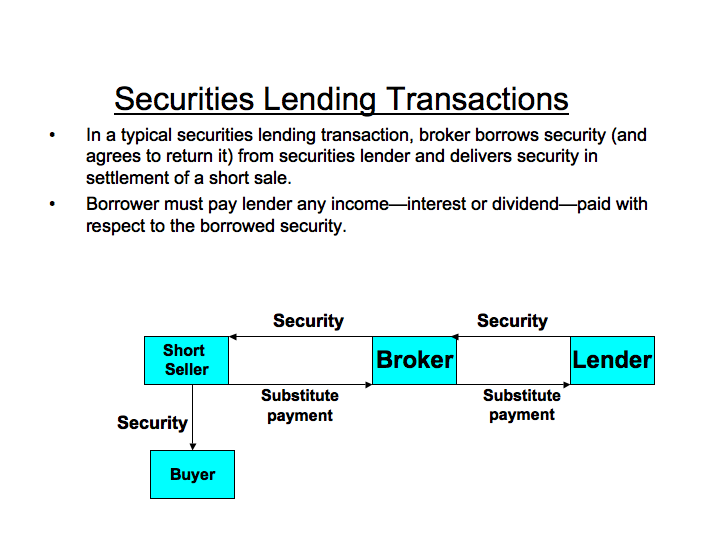
\includegraphics[width=120mm, height=70mm, clip, trim= 3mm 5mm 5mm 5mm]{seclend.png}}
\end{center}
\label{your-reference-key}
\end{figure}
Under the securities lending agreement, the borrower must pay the lender any income, such as interest or dividends, paid with respect to the borrowed security.  Under U.S. law, the substitute, or in-lieu dividend was not treated a ``dividend" for U.S. tax purposes, but rather as a fee or rent for the borrowing.  Foreign taxpayers would loan their U.S. stock over the record date and argue that the substitute dividend was not a dividend for FDAP purposes.  In addition, treaty residents argued that the income was exempt under the \emph{Other Income} article (Article 22 of the Treaty) and therefore not taxable in the source state.  

In response to these transactions, the IRS issued regulations that  adopt a look-through treatment for substitute interest and dividend payments in securities lending transactions.   Under this approach, substitute interest and dividends are sourced in the same manner as the interest or dividends accruing on the transferred security.  Reg.\@ \S\S1.861-2(a)(7) (source of substitute interest); 1.861-3(a)(6) (source of substitute dividends); 1.871-7(b)(2) (character of substitute payments); and 1.894-1(c) (treatment of substitute payments under treaties).  \margit{Substitute interest and dividend payments have the same character and source as the underlying interest or dividend.}The regulations provide that if a substitute dividend or substitute interest payment is received by a \emph{foreign person}, it has the same character as the underlying interest or dividend to which it relates for FDAP and treaty purposes. This rule has the effect of treating substitute dividends payments with respect to U.S. stock as U.S. source dividends subject to FDAP tax, but it also preserves the portfolio interest exception for substitute interest payments.

The final option employs an equity swap to avoid withholding tax.  An equity swap is a bilateral contract with a bank pursuant to which one party (for example, a bank) agrees to pay the economic appreciation with respect to a notional amount of shares of one or more companies, including both capital gain and dividends, and the other party (for example, the hedge fund) agrees to pay any depreciation with respect to the same notional amount of shares.  The party that receives the appreciation and pays depreciation is called the \emph{long party}, and the counterparty is the \emph{short party}.  The long party must also pay a financing cost that is calculated by applying an interest rate, typically LIBOR plus an additional amount, to the notional amount of the shares.  The long party thus is in the same economic position as if it had borrowed to purchase the referenced shares: it benefits by any dividend and appreciation but bears any depreciation and the financing cost of the position.

\begin{figure}[hbtp]
\caption{Equity Swap}
\begin{center}
\setlength\fboxsep{0pt}
\setlength\fboxrule{0.5pt}
\fbox{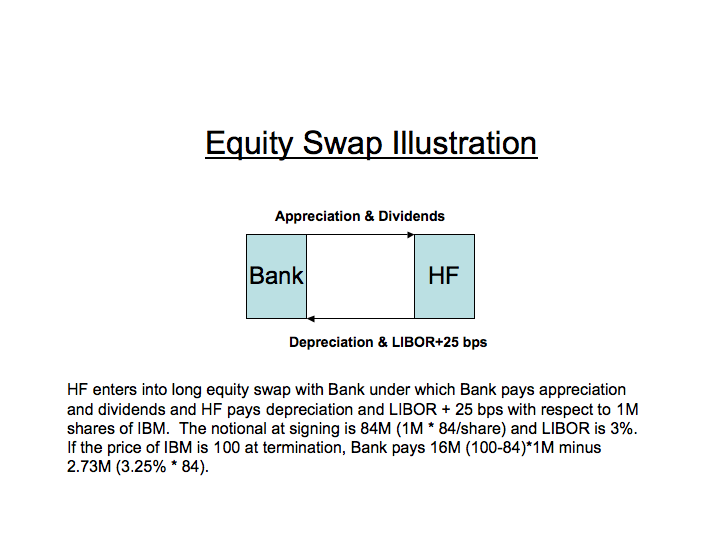
\includegraphics[width=120mm, height=80mm, clip, trim= 5mm 5mm 5mm 20mm]{equityswap.png}}
\end{center}
\label{your-reference-key}
\end{figure}

Assume that the swap payment received by a foreign hedge fund represents economically (mimics) the appreciation and dividends (less a financing charge) of a notional amount of shares of a U.S. corporation.  How should the payment be treated under section 871 or 881?  Should the gross payment be disaggregated into separate portions and the U.S. tax rules applied to each portion?  Should some portion of the swap income be U.S. source FDAP?  One issue that arises is that the payment that represents the dividend portion is generally not a dividend for U.S. tax purposes as the equity swap party does not actually own the shares and receive the payment from the dividend paying company.  Yet another issue that arises is if there is no capital gain and the financing charge offsets the notional dividend amount so that no amount is paid or received.  Also, if the swap is between two foreign parties, on what basis should the United States be able to assert tax jurisdiction over any of the payments?  Finally, would your conclusions to the questions above change if the bank had actually purchased and held the underlying shares during the term of the swap?

To encourage swap activity by U.S. banks, the IRS issued regulations in 1991 that source swap income by reference to the residence of the recipient.  Reg.\@ \S1.863-7(b)(1).  Consequently, regardless of the character of swap income, under these regulations swap income received by a foreign investor is foreign source and exempt from tax.  \margit{Swap income is generally sourced by the residence of the recipient.}That swap income representing dividends from U.S. companies was exempt from U.S. tax while the actual dividends were taxable was not lost on investment banks, who aggressively promoted swap transactions as a way for foreign hedge funds to avoid U.S. withholding tax without forgoing economic exposure to the underlying stocks.  In response to the press reports of these transactions, in 2010, Congress added new section 871(m), which provides that ``dividend equivalent payments" are treated as a U.S. source dividend for sourcing and withholding tax purposes.  A dividend equivalent payment includes substitute dividends and swap payments that are contingent upon or determined by reference to the payment of a U.S. source dividend.  


%Needless to say, the press reports of these transactions have raised concerns in Congress and the IRS.\footnote{This issue is discussed in Jeffrey M. Col\'on, \emph{Financial Products and Source Basis Taxation: U.S. International Tax Policy at the Crossroads}, 1999 University of Illinois Law Review 775 (1999)}                   

%\addcontentsline{toc}{section}{\protect\numberline{}Hedge Funds Use Swaps to Avoid Dividends} 
%\begin{select}
%\revrul{Hedge Funds Use Swaps to Avoid Dividends}{Anita Raghavan, Wall Street Journal (9/17/07)}
%
%
%Wall Street firms have long sought to use financial alchemy to save clients a bundle on their tax bills. Now, one of the Street's cleverest strategies is coming under scrutiny. 
%
%The strategy arose a few years ago, a time when lots of U.S. companies were paying fat dividends. Wall Street sensed a golden business opportunity: sell their hedge-fund clients on ways to make those dividends even fatter by avoiding taxes on them. 
%
%Bankers at Lehman Brothers Holdings Inc. pitched an enticing product. By using a complex financial tool called derivatives, hedge funds with offshore operations could reap the benefits of owning big-dividend U.S. stocks without actually owning them. The result: no dividend-tax bite. Different versions of the strategy cropped up all over Wall Street. 
%
%Hedge funds were thrilled. The Internal Revenue Service apparently wasn't. Federal tax authorities are seeking information about the trades from Lehman and Citigroup Inc., The Wall Street Journal reported in July, and other firms are bracing for similar inquiries. The government's question: Are the trades executed for any purpose other than to sidestep the dividend tax? 
%
%A look at the evolution inside Lehman of this controversial tax product shows that the firm paid considerable attention to how the IRS might react. Internal Lehman emails reviewed by the Journal reveal bankers searching for the line between smart tax planning and improper tax avoidance. In the end, according to the emails and to people familiar with Lehman's business, the bankers and their lawyers concluded that it was a business worth pursuing. 
%
%In recent years, Wall Street firms have been devising increasingly complex ways for sophisticated investors like hedge funds to minimize their tax bills. That's made it tough on tax authorities charged with deciding which maneuvers comply with tax laws and which don't. 
%
%The dividend-tax trades represent one more dimension to the spread of derivatives, complex financial instruments whose values are tied to those of assets such as stocks, commodities or currencies. Investors first turned to derivatives to hedge against risk, then as a tool to add leverage. Now, Wall Street is marketing them as a way to minimize taxes. This comes at a time when Congress is considering changing the way hedge-fund managers and private-equity firms are taxed. 
%
%The dividend-tax trades have allowed hedge funds to avoid paying more than \$1 billion a year in taxes on U.S. stock dividends, accountants and others in the business estimate. If the IRS decides the tax treatment of the trades isn't proper, it could try to slap funds with big bills for back taxes. 
%
%Nobel laureate Joseph Stiglitz, a Columbia University professor and expert witness in tax cases who examined some of the Lehman documents, says the question for tax authorities is: ``Would these trades occur at all if it were not for the tax advantages?'' If the answer is no, he says, ``at the very minimum, it is a red flag.'' 
%
%Nearly every major U.S. securities firm--from Lehman to Citigroup to Merrill Lynch \& Co.--offers such derivatives to hedge-fund clients. Foreign banks such as Germany's Deutsche Bank AG and Switzerland's UBS AG also sell the products, people familiar with the business say. 
%
%Some bankers contend that U.S. tax rules on dividends don't apply to derivatives because derivatives aren't governed by the same rules as stocks. ``We believe we are in line with industry practice as articulated by major law firms in accordance with the full knowledge of the IRS for many years,'' says John Wickham, whose job at Lehman includes overseeing the group that sells these types of derivatives. Citigroup says that the IRS views the inquiry as industrywide, and that it is cooperating. Merrill, Deutsche Bank and UBS declined to comment. 
%
%Wall Street has devised many forms of dividend-tax trades, of varying complexity. One simple kind uses a derivative called a stock swap. A Wall Street firm buys a block of stock from a hedge fund. The investment bank and the hedge fund also agree to an exchange: For a stipulated period of time, the investment bank makes payments to the hedge fund equal to the total returns on the purchased stock--the dividends plus the share appreciation--thereby simulating the benefits of actually owning the stock. In return, the hedge fund makes payments to the bank tied usually to a benchmark interest rate. If the stock declines in value, the hedge fund also must pay the bank the equivalent of the lost value. 
%
%Ordinarily, the IRS, to ensure it can collect dividend taxes from hedge funds that own U.S. stock but are domiciled outside of the country, requires securities firms to withhold the taxes from dividend payments distributed to the funds. (Domestic taxpayers are required simply to declare dividend income on their U.S. tax returns.) But when an offshore fund enters into a stock swap, who's on the hook for the dividend taxes? The U.S. banks that peddle such swaps are responsible for paying the tax, but they offset the dividend income with the expense of swap payments made to the hedge funds. The result: Because the payments received from the hedge fund are comparatively small, the bank has very little taxable income. The swap payments received by the offshore hedge fund are not subject to U.S. taxation. 
%
%The IRS declines to comment on the matter. 
%
%Hedge funds use swaps for all sorts of reasons having nothing to do with tax planning, including to lower trading costs and to make it harder for rivals to figure out what they're investing in. 
%
%The dividend-tax trading strategy became popular after changes to federal tax laws in 2003, which lowered the tax rate that individuals pay on dividends, but left the corporate rate intact. Many companies then boosted their dividend payments. European hedge funds and U.S. funds with offshore hubs jumped into these U.S. stocks, but were looking for ways to lower the tax bite. 
%
%For years, many securities firms in London, including Lehman's office there, had used derivatives to help hedge funds avoid paying a British tax known as the stamp duty, which is levied on purchases of stocks and real estate. In the summer of 2003, Richard Story, a Lehman executive in London, began pressing managers in New York to boost the volume of dividend-related derivative trades they executed, according to people familiar with the matter. 
%
%Lehman had concocted a strategy it called the Cayman Islands Trade, which offered offshore hedge funds--including the many U.S. funds with offshore operations--a way to ``enhance the yield'' on dividend-paying U.S. stocks, according to a Lehman document. The trade, which involves several legs, originates with a loan of stock from a client to a Lehman entity in the Cayman Islands. 
%
%To ascertain whether tax products will pass muster with federal tax authorities, U.S. securities firms routinely seek opinions from in-house and outside lawyers. Some legal opinions conclude that products ``will'' pass muster, while others say they ``should.'' Both grades are considered to provide acceptable legal comfort. ``More likely than not,'' a lower grade, is seen as more problematic. 
%
%``I know you got US Tax Dept (Darryl) comfortable on the Cayman yield enh. [enhancement] trades after a lot of gentle persuasion,'' Mr. Story wrote in a June 12, 2003, internal email, referring to Lehman tax attorney Darryl Steinberg. ``Did we finally get a written opinion from external counsel and if so what level of opinion was it . . . ?'' 
%
%The view from outside, at least initially, appeared fuzzy. A lawyer from Cravath, Swaine \& Moore LLP initially believed the transactions ``should'' pass muster with the IRS, according to an email to Mr. Story from Bruce Brier, a Lehman senior vice president. But after a talk with a Lehman tax lawyer, the Cravath attorney ``downgraded his opinion to `more likely than not,''' Mr. Brier wrote in the email. ``I think I can get him back to `should.'" 
%
%A Cravath spokeswoman declined to comment, as did Mr. Steinberg. Mr. Story, who no longer works at Lehman, didn't respond to requests for comment. 
%
%``You are looking at a one-page personal opinion in a thousand-page universe," a Lehman spokeswoman says. Mr. Brier's email ``in no way suggests that Cravath provided an actual written opinion and then changed it. Rather, it appears Mr. Brier and Corporate Tax were separately discussing the Cravath lawyer's possible opinion level considering a variety of different factors, some of which, when combined, would lead to a `should' level and others a `more likely than not.'" Such an exchange is ``an ordinary process of idea sharing." 
%
%Lehman touted such trades to clients in a brochure entitled ``The Power of Synthetics." The derivatives would transfer to clients ``economic exposure of a security, basket or index without taking physical ownership or delivery," the brochure said. The potential benefits included ``tax management" and ``yield enhancement," it said. 
%
%A Lehman document indicates that a number of hedge funds entered into trades, including Angelo Gordon \& Co.; Highbridge Capital Management, the big hedge fund majority-controlled by J.P. Morgan Chase \& Co.; JMG Triton; and KBC Alternative Investment Management. The Lehman document projects that the trades would save Highbridge, which has about \$37 billion in assets, about \$10.8 million in withholding taxes in 2005. JMG Triton was projected to save \$15.3 million, Angelo Gordon, \$9 million, and KBC, \$3 million, according to the document. 
%
%A KBC spokesman says, ``We have not seen that document and do not know what those numbers represent. The only reason we would track withholding taxes is if they are owed." Highbridge declined to comment. Angelo Gordon and JMG Triton didn't respond to requests for comment. 
%
%Lehman and its clients saved \$70 million in taxes they potentially owed in 2004 because of the swaps, according to the Lehman document, which refers to the withholding-tax savings as ``WHT@Risk." Lehman says the figure is from a ``draft presentation" and only represents ``one person's view of hypothetical exposure," which the firm now calls unrealistic. People familiar with Lehman's operations estimate that over the past 3 1/2; years, the firm has saved about \$200 million for its clients through such tax trades. A Lehman spokeswoman calls the figure ``conjecture." 
%
%In 2004, after Microsoft Corp. set plans to pay a one-time dividend of \$3 a share--a \$33 billion total payout--competition heated up among Wall Street firms to offer clients ways to capture a greater after-tax share of the dividend. Ian Maynard, a Lehman trading manager based in London, saw the special dividend as an opportunity for Lehman to seize business from competitors. But Lehman rivals were more aggressive, offering clients as much as 97\% of the Microsoft dividend amount compared with Lehman's 95\%, according to people familiar with the matter. 
%
%Some aspects of the business, including its profitability, worried Mr. Maynard, these people say. In a Sept. 21, 2004, email to several Lehman executives, he suggested Lehman was taking too much risk by ``guaranteeing" to pay the entire dividend amount to clients through some derivative trades. The range of clients for whom Lehman is ``guaranteeing 100\%" has ``increased significantly," he wrote. 
%
%In the email, he also noted that there appeared to be no ``consistent" standards about the minimum time clients held the derivatives, and that ``churning"--a term commonly used to refer to excessive short-term trading--appears to be ``reasonably frequent." From a tax-risk perspective, that was important. If it appeared that clients were executing such trades before dividend time, then unwinding them just after dividends were paid, tax authorities could suspect the trades were done solely to avoid taxes. 
%
%``We need to set minimum holding periods following advice from tax/compliance and eradicate any frequent churning of position," Mr. Maynard wrote. 
%
%Mr. Maynard referred questions about the matter to Lehman's spokeswoman. ``In light of evolving market conditions and technological advances," she says, ``Ian wanted to make sure that we were consistently enforcing the policies we had put in place." 
%
%Some at Lehman expressed concern over swaps tied to a single stock. Mr. Brier, the senior vice president and a tax lawyer by background, was worried the single-stock swaps could be viewed purely as a maneuver to sidestep withholding taxes, say people familiar with the situation. In an email early in 2005, he questioned whether such swaps, from a taxation standpoint, were essentially stock loans. It was a crucial question: When stocks are lent across borders, the dividend payments can be subject to taxes. 
%
%John DeRosa, Lehman's top tax official, says swaps ``possess markedly different fundamental and economic characteristics from stock loans" and thus are not subject to withholding taxes. 
%
%In a Feb. 14, 2005, email to Mr. Brier and others, Neil Sherman, a Lehman sales executive, suggested some guidelines for single-stock swaps, including that clients be required to hold them for at least 30 days. Swaps that give clients exposure to a basket of stocks could be used, he wrote, but ``care should be taken, through the observation of objective criteria, that such swaps do not have withholding tax avoidance as a principal purpose." 
%
%In a return email, Mr. Brier told Mr. Sherman it would be ``premature" to issue any new single-stock swap guidelines because, among other things, there hadn't been approval from the firm's tax department. 
%
%The Lehman spokeswoman says the directive by Mr. Sherman, who is no longer at the firm, was not triggered by any problem. Mr. Brier said recently, in a prepared statement: ``It has since come to my attention that the firm had appropriate policies in place since 2000 regarding single-equity swaps, and had previously taken legal advice from numerous outside law firms that addressed the issues which I was raising and had reached similar positive conclusions. . . . After many discussions internally and with outside counsel, it was my belief that the product was legally sound and appropriate." 
%
%At a meeting last fall of the Wall Street Tax Association, a group of tax experts, Lehman and other Wall Street firms got their first inkling that tax authorities were examining dividend-related trades, people familiar with the meeting say. Directors were buzzing about rumors of an IRS inquiry into such trades, these people say. 
%
%Todd Tuckner, UBS's tax head for the Americas, indicated that the IRS had given the bank a diagram of a transaction it appeared to be scrutinizing, the people say. After checking with the IRS, Mr. Tuckner made the diagram available to the group. Mr. Tuckner, through a spokesman, declined to comment. 
%
%Lehman still offers single-stock swaps to clients. ``Because there has been no definitive guidance to the financial community on this issue, Lehman, like its competitors, relies on its own internal analysis of the tax law and a `should'-level tax opinion from a major Wall Street law firm that clearly distinguishes our single-stock-swap trades from stock loans,'' the firm says. It declines to say which law firm provided the tax opinion. 
%\end{select}
%
%These well publicized transactions have raised concerns in Congress, which is considering changing U.S. law to treat certain swap income related to dividends on the underlying U.S. stock as U.S. source income.  

Section 871(m) is described below in an excerpt  from Joint Committee Report JCX-4-10.  The drafting of regulations implementing section 871(m) has been an arduous process because of the difficulty of finding and taxing U.S. dividend returns that are embedded in complex financial contracts, such as options and swaps.  Final regulations were issued on October 13, 2015, Reg.\@ \S1.871-15 and -15T.  These regulations were to be effective for contracts issued on or after Jan. 1, 2017.  On December 2, 2016, however, the Treasury issued Notice 2016-76, which modifies the 871(m) regulations and delays the effective date on certain complex contracts until January 1, 2018. 
 
\begin{select}
\revrul{Technical Explanation of the Revenue Provisions Contained in Senate Amendment 3310, the ``Hiring Incentives to Restore Employment Act," under Consideration by the Senate February 23, 2010.}{}

\begin{center}\textbf{Explanation of Provision}
\end{center}

The provision treats a dividend equivalent as a dividend from U.S. sources for certain purposes, including the U.S. withholding tax rules applicable to foreign persons.

A dividend equivalent is any substitute dividend made pursuant to a securities lending or a sale--repurchase transaction that (directly or indirectly) is contingent upon, or determined by reference to, the payment of a dividend from sources within the United States or any payment made under a specified notional principal contract that directly or indirectly is contingent upon, or determined by reference to, the payment of a dividend from sources within the United States. A dividend equivalent also includes any other payment that the Secretary determines is substantially similar to a payment described in the immediately preceding sentence. Under this rule, for example, the Secretary may conclude that payments under certain forward contracts or other financial contracts that reference stock of U.S. corporations are dividend equivalents.

A specified notional principal contract is any notional principal contract that has any one of the following five characteristics: (1) In connection with entering into the contract, any long party transfers the underlying security; (2) in connection with the termination of the contract, any short party transfers the underlying security to any long party; (3) the underlying security is not readily tradable on an established securities market; (4) in connection with entering into the contract, any short party to the contract posts the underlying security as collateral; or (5) the Secretary identifies the contract as a specified notional principal contract. For purposes of these characteristics, for any underlying security of any notional principal contract (1) a long party is any party to the contract that is entitled to receive any payment under the contract that is contingent upon or determined by reference to the payment of a U.S.-source dividend on the underlying security, and (2) a short party is any party to the contract that is not a long party in respect of the underlying security. An underlying security in a notional principal contract is the security with respect to which the dividend equivalent is paid. For these purposes, any index or fixed basket of securities is treated as a single security.

For payments made more than two years after the provision's date of enactment, a specified notional principal contract also includes any notional principal contract unless the Secretary determines that the contract is of a type that does not have the potential for tax avoidance.

No inference is intended as to whether the definition of specified notional principal contract, or any determination under this provision that a transaction does not have the potential for the avoidance of taxes on U.S.-source dividends, is relevant in determining whether an agency relationship exists under general tax principles or whether a foreign party to a contract should be treated as having beneficial tax ownership of the stock giving rise to U.S.-source dividends.

The payments that are treated as U.S.-source dividends under the provision are the gross amounts that are used in computing any net amounts transferred to or from the taxpayer. The example of a ``total return swap" referencing stock of a domestic corporation (an example of a notional principal contract to which the provision generally applies), illustrates the consequences of this rule. Under a typical total return swap, a foreign investor enters into an agreement with a counterparty under which amounts due to each party are based on the returns generated by a notional investment in a specified dollar amount of the stock underlying the swap. The investor agrees for a specified period to pay to the counterparty (1) an amount calculated by reference to a market interest rate (such as the London Interbank Offered Rate (``LIBOR")) on the notional amount of the underlying stock and (2) any depreciation in the value of the stock. In return, the counterparty agrees for the specified period to pay the investor (1) any dividends paid on the stock and (2) any appreciation in the value of the stock. Amounts owed by each party under this swap typically are netted so that only one party makes an actual payment. The provision treats any dividend-based amount under the swap as a payment even though any actual payment under the swap is a net amount determined in part by other amounts (for example, the interest amount and the amount of any appreciation or depreciation in value of the referenced stock). Accordingly, a counterparty to a total return swap may be obligated to withhold and remit tax on the gross amount of a dividend equivalent even though, as a result of a netting of payments due under the swap, the counterparty is not required to make an actual payment to the foreign investor.

\ldots

\end{select}

\addcontentsline{toc}{section}{\protect\numberline{}Comments}
	\begin{center}
		\textbf{\emph{Comments}}
			\end{center}



This chapter introduced the source of income rules of sections 861 and 862 for interest and dividends.  The source rules assign a source--foreign or U.S.--to items of income and expenses.  They are relevant for nonresidents because nonresidents are generally not taxed on foreign source income and for citizens and residents for purposes of the foreign tax credit rules.  The source rules do not impose any substantive tax liability, as do, for example, sections 1 and 871.  Some shady promoters and return preparers take the position that section 861 and the regulations thereunder permit a U.S. taxpayer to avoid tax on U.S. source income.  Taxpayers, even famous ones, who take such a position on a return face severe penalties and possibly imprisonment.  See Rev. Rul.  2004--30, 2004--1 C.B. 622.    
%\addcontentsline{toc}{section}{\protect\numberline{}Snipes Indicted for Tax Evasion} 
\begin{select}
	\revrul{Snipes' Sentence a Big Win for Tax Officials} 

Action star Wesley Snipes' three-year sentence on tax charges is a big win for prosecutors.

As Forbes reported earlier this week,\footnote{\url{http://bit.ly/2jyPamb}. A copy of the Snipes's amended 1997 tax return can be found at \url{http://bit.ly/2k4gnhr}} officials are increasingly concerned about a growing number of so-called ``tax defiers." Prosecutors pushed hard for a tough sentence in the Snipes case, worrying that anything less risked emboldening the movement.

Tax defiers--or ``tax protesters" as they've traditionally been known--glom onto one kooky, discredited theory or another as to why the income tax is illegal or doesn't apply to them personally or doesn't cover their normal sources of income. (Example: Only foreign income, or only earnings of federal employees are taxable.) They typically file returns showing zero income or simply stop filing. Sometimes they also put in claims for refunds on taxes they paid before their conversions, as Snipes did. 

Snipes was the highest-profile criminal tax target in years, and prosecutors called for a heavy sentence to deter others from trying to impede the IRS. The government alleged Snipes earned at least \$13.8 million in income for the years in question, on which he owed \$2.7 million in back taxes. 

Snipes was acquitted in February of five additional charges, including felony tax fraud and conspiracy. Snipes' co-defendants, Douglas P. Rosile and Eddie Ray Kahn, were convicted on both those counts. Kahn, who refused to defend himself in court, was sentenced to 10 years, while Rosile received 54 months. Both will serve three years of supervised release. Snipes will serve one year of supervised release. 

In court Thursday, Snipes read from a statement, apologizing for his ``costly mistakes," but never mentioned the word ``taxes." 
\end{select}

\addcontentsline{toc}{section}{\protect\numberline{}Interest and Dividend Problems} 
	\begin{center}
		\textbf{Interest and Dividend Problems}
	\end{center}
	\begin{select}
 	\textit{First determine the source of the item of income (sections 861-865), the taxation of the item (section 871 or 881), and finally whether the payor of the item must withhold (section 1441 or 1442).  Answer each of the problems below first assuming that the recipient is not entitled to the benefits of any income tax treaty, and then determine whether your answer would be modified by the Treaty.  Dividends and interest are addressed in Articles 10 and 11.}   
 	\begin{enumerate}
		\item Interest paid to a U.K. citizen and resident:
			\begin{enumerate} 
				\item on a corporate bond issued by Coca Cola.  The bond holder doesn't own any stock. [1441(c)(9); Reg.\@ \S 1.1441-1(b)(4)(i); and the ConAgra Foods prospectus]
				\item on a CD issued by the New York branch of Citigroup Inc., a U.S. corporation.[871(i)(2)(A); 1441(c)(10); Reg.\@ \S 1.1441-1(b)(4)(ii), -(e)(3)]
				\item on a CD issued by a U.K. branch of Citigroup. [Reg.\@ \S 1.1441-1(b)(4)(iii)]
				\item on a tax-exempt NYC municipal bond [Reg.\@\@ \S 1.861-2(a)(1)] (Regardless of the source of interest, why shouldn't foreigners generally buy U.S. tax-exempt bonds?)
				\item For each of the above questions, very briefly describe what documentation, \emph{if any}, the U.K. resident should provide to the U.S. payor.  
			\end{enumerate}
		\item A U.K. resident holds a bond of DC, a Delaware corporation, that pays annual interest of \$100.   Assume alternatively:
			\begin{enumerate}
				
				\item The bondholder owns 15\% of DC's voting stock.
				
%				\item The bondholder owns 15\% of DC's voting stock, and the first interest payment of \$100 is made during DC's first taxable year.  DC's gross income for this year consists of \$750 from a construction project in Brazil and \$250 as interest on deposits with banks in the U.S. [861(c)(1)]
%				\item The bondholder owns 15\% of DC's voting stock and DC's gross income consists of \$850 from a construction project in Brazil and \$150 as interest on deposits with banks in the U.S. [861(c)(1), (c)(2)(B)]
				\item Same as previous question, except that the U.K. resident owns 5\% of DC's stock.
				\item Same as previous question, except that the bond was guaranteed by DC's parent, a Cayman corporation.  DC defaults on an interest payment, and the Cayman corporation pays as guarantor. [Reg.\@\@ \S 1.861-2(a)(5)]
			\end{enumerate}  		
			
			\item A U.K. bank loans money to a U.K. branch of IBM, which pays interest on the loan to bank. [\S 881(a), (c)]
			
			\item A U.K. parent corporation loans money to its wholly owned U.S. subsidiary, which pays interest to the parent.
			
			\item UKPS, a U.K. partnership, owns 50\% of the stock and 20\% of the debt of USCo, a U.S. corporation.  UKPS has 100 equal partners.  USCo makes an interest payment to UKPS. [Reg.\@ \S 1.871-14(g)]
			
			\item PS, a partnership organized under U.S. law, borrows money from a Brazilian citizen.  PS carries on a trade or business in the U.S., but this business produces only a small portion of PS's income (5\%), and the borrowing has nothing to do with the U.S. business.  The Brazilian owns 15\% of PS. Note, partnerships compute their income in the same way as individuals (\S 703).  [861(a)(1), (a)(1)(B); Reg.\@ \S1.861-2(a)(2)] 
			
			\item  PS, a partnership organized under U.S. law, has only U.S. partners, and invests in start-up companies.  (Under U.S. law, such a partnership would probably \emph{not} be considered to have a U.S. trade or business.)  It borrows money from Citigroup. What is the source of the interest paid?  [Reg.\@ \S 1.861-2(a)(2)]
			
			\item U.K. resident receives a dividend from IBM.
			
			\item U.K. resident purchases debt issued by IBM that promises a fixed interest rate of 6\% per annum plus 1\% of IBM's preceding year's cash flow.  U.K. resident receives an interest payment of \$80, of which \$60 is attributable to the fixed interest rate and \$20 to the cash flow. [871(h)(4)]
			
			\item U.K. parent corporation receives a dividend from its wholly owned U.S. subsidiary.
			
			\item A U.K. pension fund receives a dividend from IBM. 
			
			\item USP, a partnership formed in the U.S. that is not engaged in a U.S. trade or business, receives a dividend from IBM.  Paul, a U.K. resident is a 10\% partner in USP.  [Reg.\@ \S 1.1441-5(b)(1), (2)(i)(A); Article 1(8)]
			
			\item UK Ltd. is a UK entity treated as a corporation for U.K. purposes but as a partnership for U.S. purposes.  This is a hybrid entity.  Paul, a U.K. resident owns 10\% of UK Ltd.  UK Ltd. receives a dividend from IBM.   [Reg.\@ \S 1.1441-5(c)(1)(i), (ii), and (iii); Article 1(8)] 
			
			\item USP, a U.S. citizen residing in London, owes money to U.K. bank and has given an interest bearing note to evidence the obligation to repay.  Now, assume that USP moves back to the U.S. and continues to pay interest on the note.  [Reg.\@ \S 301.7701(b)-1(a).]
			
%			\item UKP, a citizen and resident of the U.K., is a shareholder in FC, a U.K. corporation.  FC has gross income of \$600 each year during years 1 through 3 from a business carried on in the U.S. and had gross income for this period from foreign operations of \$400 annually.  Its taxable income effectively connected with its domestic business was \$60 per year, and foreign business profits were \$100 per year.  Late in year 3, FC received a dividend of \$600 from a foreign subsidiary that derives all of its income from businesses carried on outside the United States.  FC then distributed the \$600 to its shareholders a few weeks later in year 3.  How would your answer change if the distribution occurred in year 4? [861(a)(2)(B); 871(i)(2)(D)]
			
			\item UKP, a U.K. citizen and resident, owns a share of IBM.  UKP loans the stock to B, a U.S. broker/dealer, under a securities lending transaction, who sells it to C, a U.S. institutional investor.  B posts with UKP the sales proceeds as cash collateral.  This amount is adjusted daily to reflect changes in the value of the IBM stock.  Thus, if IBM rises, B pays UKP, and vice versa.  UKP pays interest on the cash collateral equal to the market rate less 50 basis points.  A dividend of \$100 per share is paid by IBM on the stock, and, pursuant to the lending agreement, \$100 is remitted to UKP as a substitute dividend payment.  What are the U.S. tax consequences to UKP?  [\S871(m); Reg.\@ \S1.894-1(c); and Article 22.]	
			
				\item Same initial facts as previous question, except that UKP sells the stock directly to C and enters into an equity swap with B, under which B pays to UKP any increase in the value of IBM stock (daily, quarterly, or yearly) and any dividends paid during the period of the swap, and UKP pays to B an amount reflecting the market rate of interest on a notional principal amount equal to the value (measured daily, quarterly or yearly) of the IBM stock, and any decrease in the value of the stock.  A \$100 dividend is paid by IBM and B pays UKP \$100 less \$5 of financing costs.  (It would be a very fruitful exercise to compare the economic returns UKP would earn if the stock went up or down by \$100 assuming that (1) he actually owned it;  (2) he was a party to the above swap contract; (3) or he loaned out the stock in a securities lending transaction.)  Assume the current price is \$300 per share.  What are the U.S. tax consequences to UKP? [\S871(m); Reg.\@ \S1.894-1; and Article 22.]
 \end{enumerate}
 	\end{select}

\begin{framed}
	\center{Last revised Aug. 23, 2015; source\_IntDiv\_Jan17\_17}
	\end{framed}